%%%%%%%%%%%%%%%%%%%%%%%%%%%%%%%%%%%%%%%%%%%
%
% From a template maintained at https://github.com/jamesrobertlloyd/cbl-tikz-poster
%
% Code near the top should be fairly standard and not need to be changed
%  - except for the document class
% Code lower down is more likely to be customised
%
%%%%%%%%%%%%%%%%%%%%%%%%%%%%%%%%%%%%%%%%%%%

%%%%%%%%%%%%%%%%%%%%%%%%%%%%%%%%%%%%%%%%%%%
%
% Document class
%
% Change this if you want a different size / orientation poster etc
%
%%%%%%%%%%%%%%%%%%%%%%%%%%%%%%%%%%%%%%%%%%%

\documentclass[landscape,a0b,final,a4resizeable]{a0poster}
%\documentclass[portrait,a0b,final,a4resizeable]{a0poster}

%%%%%%%%%%%%%%%%%%%%%%%%%%%%%%%%%%%%%%%%%%%
%
% 'Basic' packages
%
% TODO - Almost certainly some are unnecessary - feel free to remove nonstandard
% packages if you think it is a good idea not to always have them
%
%%%%%%%%%%%%%%%%%%%%%%%%%%%%%%%%%%%%%%%%%%%

\usepackage{multicol}
\usepackage{color}
\usepackage{shadow}
\usepackage{morefloats}
\usepackage{cite}
\usepackage[pdftex]{graphicx}
\usepackage{rotating}
\usepackage{amsmath, amsthm, amssymb, bm}
\usepackage{array}
\usepackage{nth}
\usepackage[square,numbers]{natbib}
\usepackage{booktabs}

%%%%%%%%%%%%%%%%%%%%%%%%%%%%%%%%%%%%%%%%%%%
%
% TIKZ packages and common definitions
%
% Add extra things as per your tikz needs
%
%%%%%%%%%%%%%%%%%%%%%%%%%%%%%%%%%%%%%%%%%%%

\usepackage{../common/picins}
\usepackage{tikz}
\usetikzlibrary{shapes.geometric,arrows,chains,matrix,positioning,scopes,calc}
\tikzstyle{mybox} = [draw=white, rectangle]

%%%%%%%%%%%%%%%%%%%%%%%%%%%%%%%%%%%%%%%%%%%
%
% myfig
%
% \myfig - replacement for \figure
% necessary, since in multicol-environment 
% \figure won't work        
%                 
%%%%%%%%%%%%%%%%%%%%%%%%%%%%%%%%%%%%%%%%%%%

\newcommand{\myfig}[3][0]{
\begin{center}
  \vspace{1.5cm}
  \includegraphics[width=#3\hsize,angle=#1]{#2}
  \nobreak\medskip
\end{center}}

%%%%%%%%%%%%%%%%%%%%%%%%%%%%%%%%%%%%%%%%%%%
%
% mycaption                
%
% \mycaption - replacement for \caption
% necessary, since in multicol-environment \figure and
% therefore \caption won't work
%
%%%%%%%%%%%%%%%%%%%%%%%%%%%%%%%%%%%%%%%%%%%

%\newcounter{figure}
\setcounter{figure}{1}
\newcommand{\mycaption}[1]{
  \vspace{0.5cm}
  \begin{quote}
    {{\sc Figure} \arabic{figure}: #1}
  \end{quote}
  \vspace{1cm}
  \stepcounter{figure}
}

%%%%%%%%%%%%%%%%%%%%%%%%%%%%%%%%%%%%%%%%%%%
%
% Some standard colours
%
%%%%%%%%%%%%%%%%%%%%%%%%%%%%%%%%%%%%%%%%%%%

\definecolor{camlightblue}{rgb}{0.601 , 0.8, 1}
\definecolor{camdarkblue}{rgb}{0, 0.203, 0.402}
\definecolor{camred}{rgb}{1, 0.203, 0}
\definecolor{camyellow}{rgb}{1, 0.8, 0}
\definecolor{lightblue}{rgb}{0, 0, 0.80}
\definecolor{white}{rgb}{1, 1, 1}
\definecolor{whiteblue}{rgb}{0.80, 0.80, 1}

%%%%%%%%%%%%%%%%%%%%%%%%%%%%%%%%%%%%%%%%%%%
%
% Some look and feel definitions
%
%%%%%%%%%%%%%%%%%%%%%%%%%%%%%%%%%%%%%%%%%%%

\setlength{\columnsep}{0.03\textwidth}
\setlength{\columnseprule}{0.0018\textwidth}
\setlength{\parindent}{0.0cm}

%%%%%%%%%%%%%%%%%%%%%%%%%%%%%%%%%%%%%%%%%%%
%
% \mysection - replacement for \section*
% 
% Puts a pretty box around some text
% TODO - any other thoughts for what this box should look like
%
%%%%%%%%%%%%%%%%%%%%%%%%%%%%%%%%%%%%%%%%%%%

\tikzstyle{mysection} = [rectangle, 
									draw=none, 
									shade, 
									outer color=camlightblue!30,
									inner color=camlightblue!30,
									text width=0.965\columnwidth,
									text centered,
									rounded corners=20pt,
									minimum height=0.11\columnwidth]

\newcommand{\mysection}[1]
{
\begin{center}
  \begin{tikzpicture}
    \node[mysection] {\sffamily\bfseries\LARGE#1};
  \end{tikzpicture}
\end{center}
}

%%%%%%%%%%%%%%%%%%%%%%%%%%%%%%%%%%%%%%%%%%%
%
% Set the font
%
% TODO - Not sure what a canonical choice is - feel free to modify
%
%%%%%%%%%%%%%%%%%%%%%%%%%%%%%%%%%%%%%%%%%%%

\renewcommand{\familydefault}{cmss}
\sffamily

%%%%%%%%%%%%%%%%%%%%%%%%%%%%%%%%%%%%%%%%%%%
%
% Poster environment
%
% Centres everything and can be used to define the width of the content
%
%%%%%%%%%%%%%%%%%%%%%%%%%%%%%%%%%%%%%%%%%%%

\newenvironment{poster}{
  \begin{center}
  \begin{minipage}[c]{0.96\textwidth}
}{
  \end{minipage} 
  \end{center}
}

%%%%%%%%%%%%%%%%%%%%%%%%%%%%%%%%%%%%%%%%%%%
%
% This is probably a good place to put content specific packages and definitions
%
%%%%%%%%%%%%%%%%%%%%%%%%%%%%%%%%%%%%%%%%%%%

\newtheorem{thm}{Theorem}%[section]
\newtheorem{lem}[thm]{Lemma}
\newtheorem{prop}[thm]{Proposition}
\newtheorem{cor}[thm]{Corollary}

\newtheorem*{theorem*}{Theorem}

\theoremstyle{definition}
\newtheorem*{definition*}{Definition}
\newtheorem{definition}[thm]{Definition}%[section]
\newtheorem{conj}{Conjecture}[section]
\newtheorem{exmp}{Example}[section]
\newtheorem{rem}[thm]{Remark}

\theoremstyle{remark}
%\newtheorem{rem}{Remark}
\newtheorem{note}{Note}
\newtheorem{case}{Case}

\newcommand{\eqd}{\overset{\,_{\!d}}{=}}
\newcommand{\defn}[1]{\emph{#1}}

\newcommand{\Law}{\mathcal{L}}

\def\given{\,|\,}

\def\SGinf{\mathbb{S}_{\infty}}

\newcommand{\NonNegInts}{\mathbb{Z}_+}
\newcommand{\Nats}{\mathbb{N}}
\newcommand{\Rationals}{\mathbb{Q}}
\newcommand{\Reals}{\mathbb{R}}

\newcommand{\as}{\textrm{a.s.}}

\def\[#1\]{\begin{align}#1\end{align}}
\newcommand{\defas}{:=}

\newcommand{\Normal}{\mathcal{N}}
\newcommand{\dist}{\ \sim\ }

\newcommand{\kernel}{\kappa}
\newcommand{\kernelmatrix}{K}
\newcommand{\scalefactor}{s}
\newcommand{\lengthscale}{\ell}
\newcommand{\targets}{T}
\newcommand{\noise}{\sigma_\targets}
\newcommand{\pseudopoints}{\eta}
\newcommand{\inputpoints}{\xi}
\newcommand{\covhyppar}{\psi}
\newcommand{\logistic}{\phi}

\newcommand{\CompOrder}{\mathcal{O}}
\def\graphspace{\mathbf{G}}
\def\Uniform{\mbox{\rm Uniform}}
\def\Bernoulli{\mbox{\rm Bernoulli}}
\def\ie{i.e.,\ }
\def\eg{e.g.,\ }
\def\iid{i.i.d.\ }
\def\simiid{\sim_{\mbox{\tiny iid}}}
\def\simind{\sim_{\mbox{\tiny ind}}}
\def\eqdist{\stackrel{\mbox{\tiny d}}{=}}
\def\ahfunction{\theta}       
\def\AHfunction{\Theta}           % A-H random function
\def\AHvar{U}                     % A-H uniform variables
\def\AHvaralt{V}                  % A-H uniform variables - for bipartite data
\def\larray{W}                    % latent array sampled with A-H
%\def\latentspace{\mathbf{W}}      % range of entries
\def\latentspace{\mathcal{W}}      % range of entries
\def\darray{X}                    % data array
%\def\dataspace{\mathbf{X}}        % sample space
\def\dataspace{\mathcal{X}}        % sample space
\def\cfspace{\mathbf{C}}          % space of continuous functions
%\def\GP{\mbox{\mathcal{GP}}}
\def\GP{\mathcal{GP}}
\def\likelihood{P}
\def\CovData{C}
\def\CovDataAlt{D}

\def\newarrow{\mbox{\begin{tikzpicture}
             \useasboundingbox{(-3pt,-4.5pt) rectangle (19pt,1pt)};
             \draw[->] (0,-0.07)--(17pt,-0.07);\end{tikzpicture}}}

%%%%%%%%%%%%%%%%%%%%%%%%%%%%%%%%%%%%%%%%%%%
%
% The document environment starts here
%
%%%%%%%%%%%%%%%%%%%%%%%%%%%%%%%%%%%%%%%%%%%

\begin{document}

%%%%%%%%%%%%%%%%%%%%%%%%%%%%%%%%%%%%%%%%%%%
%
% Begin the poster environment - centres things and potentially changes the width
%
%%%%%%%%%%%%%%%%%%%%%%%%%%%%%%%%%%%%%%%%%%%

\begin{poster}

%%%%%%%%%%%%%%%%%%%%%%%%%%%%%%%%%%%%%%%%%%%
%
% Potentially add some space at the top of the poster
%
%%%%%%%%%%%%%%%%%%%%%%%%%%%%%%%%%%%%%%%%%%%

\vspace{0\baselineskip}

%%%%%%%%%%%%%%%%%%%%%%%%%%%%%%%%%%%%%%%%%%%
%
% Draw the header as a TIKZ picture
%
% Using TIKZ to allow for easy alignment
%
%%%%%%%%%%%%%%%%%%%%%%%%%%%%%%%%%%%%%%%%%%%

\begin{center}
\begin{tikzpicture}[x=0.5\textwidth]
    % Dummy nodes at edges for spacing
    % TODO - a better way?
    \node at (+1, 0) {};    
    \node at (-1, 0) {};
    % Set the size of the badges
    \def \badgeheight {0.08\textwidth}
    % Title text
    \node[inner sep=0,text width=0.5\textwidth,text centered,font=\Huge] (Title) at (0,0) 
    {
      {\sffamily \Huge \textbf{Estimating Convergence of Markov chains with\\\(L\)-Lag Couplings}}\\
      {\huge\sffamily Niloy Biswas\textsuperscript{1}, Pierre E. Jacob\textsuperscript{1}, Paul Vanetti\textsuperscript{2}}\\
      \vspace{-0.3\baselineskip}
      {\Large\sffamily 1: Harvard University 2: University of Oxford}
    };
    % Harvard badge
    \node [mybox] (Cambridge Badge) at (-0.9, 0) {
        \includegraphics[height=0.1\textwidth]{../badges/harvard.png}
    };

    % QR Code
    \node [mybox] (QR Code Badge) at (0.375, -1.9) {
        \includegraphics[height=0.05\textwidth]{../badges/LlagCouplingsQRCode.png}
    };
    
    % Oxford badge
    \node [mybox] (box) at (0.875, 0) {
        \includegraphics[width=0.1\textwidth]{../badges/oxford.png}
    };
\end{tikzpicture}
\end{center}

%%%%%%%%%%%%%%%%%%%%%%%%%%%%%%%%%%%%%%%%%%%
%
% Spacing between title and main body
%
%%%%%%%%%%%%%%%%%%%%%%%%%%%%%%%%%%%%%%%%%%%

\vspace{-1.75\baselineskip}

%%%%%%%%%%%%%%%%%%%%%%%%%%%%%%%%%%%%%%%%%%%
%
% Columns environment
%
%%%%%%%%%%%%%%%%%%%%%%%%%%%%%%%%%%%%%%%%%%%

\begin{multicols}{3}

%%%%%%%%%%%%%%%%%%%%%%%%%%%%%%%%%%%%%%%%%%%
%
% Start of content
%
%%%%%%%%%%%%%%%%%%%%%%%%%%%%%%%%%%%%%%%%%%%

\large

\mysection{Motivation: \\ Measure non-asymptotic bias of MCMC}

\vspace{0.3\baselineskip}

{\Large \begin{itemize}
\item MCMC methods have \textbf{non-asymptotic bias}: they only reach a target distribution as the number of iterations goes to infinity.
\vspace{1\baselineskip}
\item We introduce \textbf{\(L\)-lag couplings} to \textbf{generate computable, non-asymptotic} \textbf{upper bound estimates for the} \textbf{total variation and} \textbf{1-Wasserstein distances} of general Markov chains to stationarity.
\vspace{0.5\baselineskip}
\begin{itemize}
\item Total Variation Distance: e.g. histograms, credible intervals
\[d_{TV}(P, Q) = \underset{\substack{h: |h|\leq 1\\ X \sim P, Y\sim Q}}{sup} \big| \mathbb{E}[h(X) - h(Y)] \big| \]
\item 1--Wasserstein: e.g. all first moments
\[d_{\text{W}}(P, Q) = \underset{\substack{h: \| h(x)-h(y) \| \leq \| x -y \| \\ X \sim P, Y\sim Q}}{sup} \big| \mathbb{E}[h(X) - h(Y)] \big| \]
\end{itemize}
\end{itemize}}

\vspace{1\baselineskip}

\mysection{What are \(L\)-Lag Couplings?}

\vspace{0.5\baselineskip}

{\Large \begin{itemize}
\item A pair of Markov chains \((X_t, Y_t)_{t \geq 0}\) such that:
\begin{itemize}
\item Same marginal distributions: 
\( X_t \sim Y_t \sim \pi_t \ \forall t \geq 0 \ \text{ with } \pi_t \overset{t \rightarrow \infty}{\Rightarrow} \pi \)
\item \(X_t\) and \(Y_{t-L}\) meet \textit{\underline{\textbf{exactly}}} at time 
\begin{equation}
\tau^{(L)}:= \inf \{ t > L : X_t = Y_{t-L} \}  \nonumber
\end{equation}
\item Chains stay faithful after coupling: \(X_t = Y_{t-L} \ \forall t \geq \tau^{(L)} \)
\end{itemize}
\end{itemize}}

\vspace{1\baselineskip}
{\Large \begin{itemize}
\item Example: 150-Lag Coupling of Random-Walk Metropolis--Hastings with start \(\delta_{10}\) and target \(\mathcal{N}(0,1)\)
\end{itemize}}

\vspace{1\baselineskip}

\begin{center}
\includegraphics[width=0.25\paperwidth]{../misc/rwmh_standard_normal_lag_150_trajectory.pdf}
\end{center}

\vspace{1\baselineskip}

{\Large \begin{itemize}
\item Coupling algorithms for common MCMC methods available (e.g. RWMH, Gibbs samplers, HMC, Particle Gibbs)
\end{itemize}}

%\begin{center}
%\input{../misc/exchangeable.tex}
%\end{center}

%\vspace{\baselineskip}

%\begin{center}
%{\Large When the labelling of nodes is arbitrary, the two adjacency matrices should be treated equivalently.}
%\end{center}

\vspace{1\baselineskip}

\newpage

\mysection{Main Theorem}

\vspace{0.25\baselineskip}

{\Large
\begin{theorem*}
Consider an \(L\)-lag coupling of chains \((X_t, Y_t)_{t \geq 0}\), where \( X_t \overset{t \rightarrow \infty}{\Rightarrow} \pi\) and 
meeting time \(\tau^{(L)}:= inf \{ t > L : X_t = Y_{t-L} \} \) has sub-exponential tails. Then, 
\begin{equation}
\boldsymbol{d_{\text{TV}}(\pi_t, \pi) \leq  \mathbb{E} \Big[ \max(0, \bigl\lceil \frac{\tau^{(L)} - L -t}{L} \bigr\rceil) \Big]}
\end{equation}
Further assume for some \(\eta >0\), \((2+\eta)\)-moments of chain \((X_t)_{t \geq 0}\) are uniformly bounded. Then, 
\begin{equation}
\boldsymbol{d_{\text{W}}(\pi_t, \pi) \leq   \mathbb{E} \Big[ \sum_{j=1}^{ \bigl\lceil \frac{\tau^{(L)} - L -t}{L} \bigr\rceil }  \| X_{t+jL} - Y_{t+(j-1)L} \|_1 \Big]}
\end{equation}
\end{theorem*}
}

\vspace{1\baselineskip}

\mysection{Stylized Example}

\vspace{0.5\baselineskip}

{\Large \begin{itemize}
\item Random-Walk Metropolis--Hastings: start \(\delta_{10}\), target \(\mathcal{N}(0,1)\)
\end{itemize}}

\vspace{0.5\baselineskip}

\begin{center}
\includegraphics[width=0.25\paperwidth]{../misc/bound_standard_normal_vertical.pdf}
\end{center}

\vspace{1\baselineskip}

\newpage

\mysection{Ising Model: Single-site Gibbs vs. Parallel Tempering}

{\Large \begin{itemize}
\item Discrete state space: \( \{-1,1 \}^{32 \times 32} \). 
\item Target: \( \pi_\beta(x) \propto \exp (\beta \sum_{i \sim j} x_i x_j) \) for all \( i \sim j \) neighboring sites. 
\end{itemize}}

\begin{center}
\includegraphics[width=0.2425\paperwidth]{../misc/ising_ssg_versus_pt.pdf}
\end{center}

\mysection{Bayesian Logistic Regression: \\ HMC vs. P\'olya-Gamma}

{\Large \begin{itemize}
\item Sampling from the posterior:
\begin{itemize}
\item Hamiltonian Monte Carlo (HMC) with parameters \(\epsilon_{HMC}, S_{HMC} \)
\item Parameter-free P\'olya-Gamma (PG)
\end{itemize}
\end{itemize}}

\begin{center}
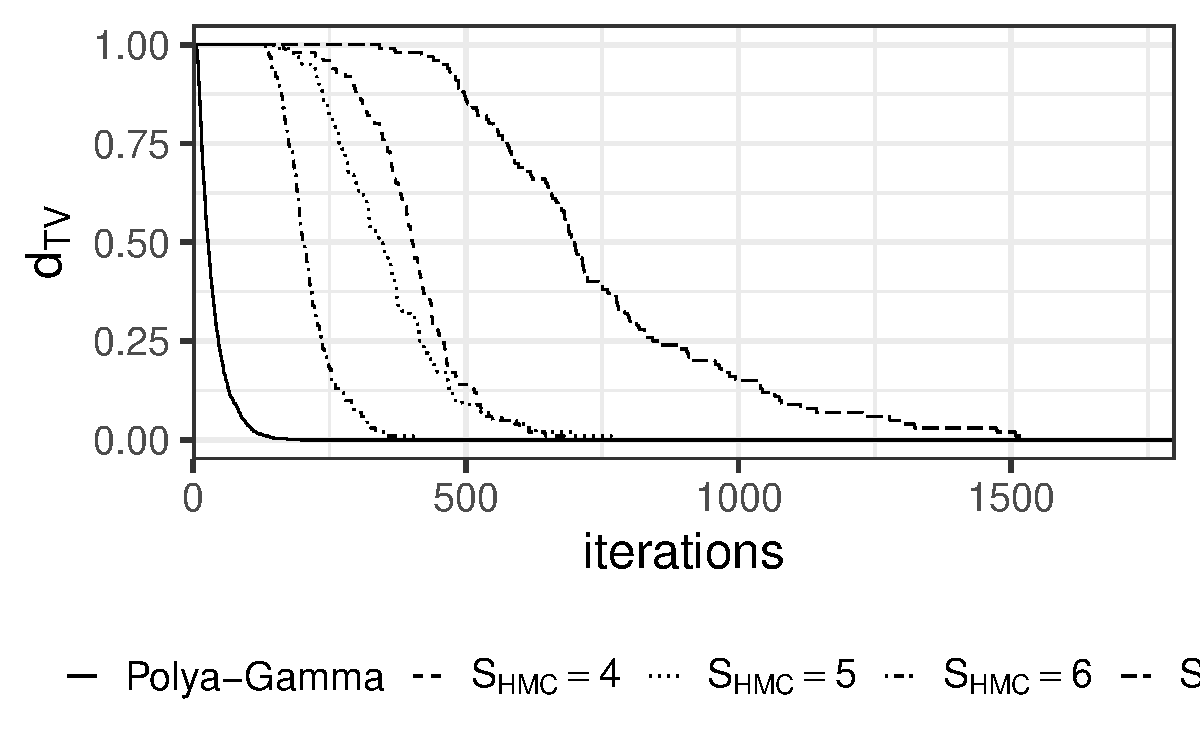
\includegraphics[width=0.2425\paperwidth]{../misc/pg_vs_hmc_small_p.pdf}
\end{center}

\mysection{References and Implementation}
{\Large 
\begin{itemize}
\item Jacob, O’Leary and Atchad\'e. Unbiased Markov chain Monte Carlo with couplings. \textit{JRSS-B}, 2019.
\item Heng and Jacob. Unbiased HMC with couplings. \textit{Biometrika}, 2019.
\item \(L\)-Lag Couplings Code: https://github.com/niloyb/LlagCouplings
\end{itemize}}

\vspace{\baselineskip}

%\begin{center}
%  \begin{tabular}{r | r r r | r r r | r r r}
%    \multicolumn{10}{c}{AUC results} \\
%    \addlinespace[2pt]
%    Data set & \multicolumn{3}{c|}{High school} & \multicolumn{3}{c|}{NIPS} & \multicolumn{3}{c}{Protein} \\
%    Latent dim. & 1 & 2 & 3 & 1 & 2 & 3 & 1 & 2 & 3 \\
%    \midrule
%    PMF                   & 0.747 & 0.792 & 0.792 & 0.729 & 0.789 & 0.820 & 0.787 & 0.810 & 0.841 \\
%    Eigenmodel            & 0.742 & 0.806 & 0.806 & 0.789 & 0.818 & 0.845 & 0.805 & 0.866 & 0.882 \\
%    GPLVM                 & 0.744 & 0.775 & 0.782 & 0.888 & 0.876 & 0.883 & 0.877 & 0.883 & 0.873 \\
%    RFM & \textbf{0.815} & \textbf{0.827} & \textbf{0.820} & \textbf{0.907} & \textbf{0.914} & \textbf{0.919} & \textbf{0.903} & \textbf{0.910} & \textbf{0.912}
%  \end{tabular}
%\end{center}

%\small{
%\bibliographystyle{unsrt}
%\bibliographystyle{../misc/natbib}
%\bibliography{misc/library,misc/biblio,misc/bibdesk-porbanz}
%}

\end{multicols}

\end{poster}

\end{document}
